
%% bare_conf.tex
%% V1.3
%% 2007/01/11
%% by Michael Shell
%% See:
%% http://www.michaelshell.org/
%% for current contact information.
%%
%% This is a skeleton file demonstrating the use of IEEEtran.cls
%% (requires IEEEtran.cls version 1.7 or later) with an IEEE conference paper.
%%
%% Support sites:
%% http://www.michaelshell.org/tex/ieeetran/
%% http://www.ctan.org/tex-archive/macros/latex/contrib/IEEEtran/
%% and
%% http://www.ieee.org/

%%*************************************************************************
%% Legal Notice:
%% This code is offered as-is without any warranty either expressed or
%% implied; without even the implied warranty of MERCHANTABILITY or
%% FITNESS FOR A PARTICULAR PURPOSE!
%% User assumes all risk.
%% In no event shall IEEE or any contributor to this code be liable for
%% any damages or losses, including, but not limited to, incidental,
%% consequential, or any other damages, resulting from the use or misuse
%% of any information contained here.
%%
%% All comments are the opinions of their respective authors and are not
%% necessarily endorsed by the IEEE.
%%
%% This work is distributed under the LaTeX Project Public License (LPPL)
%% ( http://www.latex-project.org/ ) version 1.3, and may be freely used,
%% distributed and modified. A copy of the LPPL, version 1.3, is included
%% in the base LaTeX documentation of all distributions of LaTeX released
%% 2003/12/01 or later.
%% Retain all contribution notices and credits.
%% ** Modified files should be clearly indicated as such, including  **
%% ** renaming them and changing author support contact information. **
%%
%% File list of work: IEEEtran.cls, IEEEtran_HOWTO.pdf, bare_adv.tex,
%%                    bare_conf.tex, bare_jrnl.tex, bare_jrnl_compsoc.tex
%%*************************************************************************

% *** Authors should verify (and, if needed, correct) their LaTeX system  ***
% *** with the testflow diagnostic prior to trusting their LaTeX platform ***
% *** with production work. IEEE's font choices can trigger bugs that do  ***
% *** not appear when using other class files.                            ***
% The testflow support page is at:
% http://www.michaelshell.org/tex/testflow/



% Note that the a4paper option is mainly intended so that authors in
% countries using A4 can easily print to A4 and see how their papers will
% look in print - the typesetting of the document will not typically be
% affected with changes in paper size (but the bottom and side margins will).
% Use the testflow package mentioned above to verify correct handling of
% both paper sizes by the user's LaTeX system.
%
% Also note that the "draftcls" or "draftclsnofoot", not "draft", option
% should be used if it is desired that the figures are to be displayed in
% draft mode.
%
\documentclass[conference]{IEEEtran}
% Add the compsoc option for Computer Society conferences.
%
% If IEEEtran.cls has not been installed into the LaTeX system files,
% manually specify the path to it like:
% \documentclass[conference]{../sty/IEEEtran}
\usepackage[english]{babel}
\usepackage[utf8]{inputenc}
\usepackage[pdftex]{graphicx}

%\usepackage{refcheck}


% Some very useful LaTeX packages include:
% (uncomment the ones you want to load)


% *** MISC UTILITY PACKAGES ***
%
%\usepackage{ifpdf}
% Heiko Oberdiek's ifpdf.sty is very useful if you need conditional
% compilation based on whether the output is pdf or dvi.
% usage:
% \ifpdf
%   % pdf code
% \else
%   % dvi code
% \fi
% The latest version of ifpdf.sty can be obtained from:
% http://www.ctan.org/tex-archive/macros/latex/contrib/oberdiek/
% Also, note that IEEEtran.cls V1.7 and later provides a builtin
% \ifCLASSINFOpdf conditional that works the same way.
% When switching from latex to pdflatex and vice-versa, the compiler may
% have to be run twice to clear warning/error messages.






% *** CITATION PACKAGES ***
%
%\usepackage{cite}
% cite.sty was written by Donald Arseneau
% V1.6 and later of IEEEtran pre-defines the format of the cite.sty package
% \cite{} output to follow that of IEEE. Loading the cite package will
% result in citation numbers being automatically sorted and properly
% "compressed/ranged". e.g., [1], [9], [2], [7], [5], [6] without using
% cite.sty will become [1], [2], [5]--[7], [9] using cite.sty. cite.sty's
% \cite will automatically add leading space, if needed. Use cite.sty's
% noadjust option (cite.sty V3.8 and later) if you want to turn this off.
% cite.sty is already installed on most LaTeX systems. Be sure and use
% version 4.0 (2003-05-27) and later if using hyperref.sty. cite.sty does
% not currently provide for hyperlinked citations.
% The latest version can be obtained at:
% http://www.ctan.org/tex-archive/macros/latex/contrib/cite/
% The documentation is contained in the cite.sty file itself.




% *** GRAPHICS RELATED PACKAGES ***
%
\ifCLASSINFOpdf
  % \usepackage[pdftex]{graphicx}
  % declare the path(s) where your graphic files are
  % \graphicspath{{../pdf/}{../jpeg/}}
  % and their extensions so you won't have to specify these with
  % every instance of \includegraphics
  % \DeclareGraphicsExtensions{.pdf,.jpeg,.png}
\else
  % or other class option (dvipsone, dvipdf, if not using dvips). graphicx
  % will default to the driver specified in the system graphics.cfg if no
  % driver is specified.
  % \usepackage[dvips]{graphicx}
  % declare the path(s) where your graphic files are
  % \graphicspath{{../eps/}}
  % and their extensions so you won't have to specify these with
  % every instance of \includegraphics
  % \DeclareGraphicsExtensions{.eps}
\fi
% graphicx was written by David Carlisle and Sebastian Rahtz. It is
% required if you want graphics, photos, etc. graphicx.sty is already
% installed on most LaTeX systems. The latest version and documentation can
% be obtained at:
% http://www.ctan.org/tex-archive/macros/latex/required/graphics/
% Another good source of documentation is "Using Imported Graphics in
% LaTeX2e" by Keith Reckdahl which can be found as epslatex.ps or
% epslatex.pdf at: http://www.ctan.org/tex-archive/info/
%
% latex, and pdflatex in dvi mode, support graphics in encapsulated
% postscript (.eps) format. pdflatex in pdf mode supports graphics
% in .pdf, .jpeg, .png and .mps (metapost) formats. Users should ensure
% that all non-photo figures use a vector format (.eps, .pdf, .mps) and
% not a bitmapped formats (.jpeg, .png). IEEE frowns on bitmapped formats
% which can result in "jaggedy"/blurry rendering of lines and letters as
% well as large increases in file sizes.
%
% You can find documentation about the pdfTeX application at:
% http://www.tug.org/applications/pdftex





% *** MATH PACKAGES ***
%
%\usepackage[cmex10]{amsmath}
% A popular package from the American Mathematical Society that provides
% many useful and powerful commands for dealing with mathematics. If using
% it, be sure to load this package with the cmex10 option to ensure that
% only type 1 fonts will utilized at all point sizes. Without this option,
% it is possible that some math symbols, particularly those within
% footnotes, will be rendered in bitmap form which will result in a
% document that can not be IEEE Xplore compliant!
%
% Also, note that the amsmath package sets \interdisplaylinepenalty to 10000
% thus preventing page breaks from occurring within multiline equations. Use:
%\interdisplaylinepenalty=2500
% after loading amsmath to restore such page breaks as IEEEtran.cls normally
% does. amsmath.sty is already installed on most LaTeX systems. The latest
% version and documentation can be obtained at:
% http://www.ctan.org/tex-archive/macros/latex/required/amslatex/math/





% *** SPECIALIZED LIST PACKAGES ***
%
%\usepackage{algorithmic}
% algorithmic.sty was written by Peter Williams and Rogerio Brito.
% This package provides an algorithmic environment fo describing algorithms.
% You can use the algorithmic environment in-text or within a figure
% environment to provide for a floating algorithm. Do NOT use the algorithm
% floating environment provided by algorithm.sty (by the same authors) or
% algorithm2e.sty (by Christophe Fiorio) as IEEE does not use dedicated
% algorithm float types and packages that provide these will not provide
% correct IEEE style captions. The latest version and documentation of
% algorithmic.sty can be obtained at:
% http://www.ctan.org/tex-archive/macros/latex/contrib/algorithms/
% There is also a support site at:
% http://algorithms.berlios.de/index.html
% Also of interest may be the (relatively newer and more customizable)
% algorithmicx.sty package by Szasz Janos:
% http://www.ctan.org/tex-archive/macros/latex/contrib/algorithmicx/




% *** ALIGNMENT PACKAGES ***
%
%\usepackage{array}
% Frank Mittelbach's and David Carlisle's array.sty patches and improves
% the standard LaTeX2e array and tabular environments to provide better
% appearance and additional user controls. As the default LaTeX2e table
% generation code is lacking to the point of almost being broken with
% respect to the quality of the end results, all users are strongly
% advised to use an enhanced (at the very least that provided by array.sty)
% set of table tools. array.sty is already installed on most systems. The
% latest version and documentation can be obtained at:
% http://www.ctan.org/tex-archive/macros/latex/required/tools/


%\usepackage{mdwmath}
%\usepackage{mdwtab}
% Also highly recommended is Mark Wooding's extremely powerful MDW tools,
% especially mdwmath.sty and mdwtab.sty which are used to format equations
% and tables, respectively. The MDWtools set is already installed on most
% LaTeX systems. The lastest version and documentation is available at:
% http://www.ctan.org/tex-archive/macros/latex/contrib/mdwtools/


% IEEEtran contains the IEEEeqnarray family of commands that can be used to
% generate multiline equations as well as matrices, tables, etc., of high
% quality.


%\usepackage{eqparbox}
% Also of notable interest is Scott Pakin's eqparbox package for creating
% (automatically sized) equal width boxes - aka "natural width parboxes".
% Available at:
% http://www.ctan.org/tex-archive/macros/latex/contrib/eqparbox/




\usepackage{footnote}
% *** SUBFIGURE PACKAGES ***
%\usepackage[tight,footnotesize]{subfigure}
% subfigure.sty was written by Steven Douglas Cochran. This package makes it
% easy to put subfigures in your figures. e.g., "Figure 1a and 1b". For IEEE
% work, it is a good idea to load it with the tight package option to reduce
% the amount of white space around the subfigures. subfigure.sty is already
% installed on most LaTeX systems. The latest version and documentation can
% be obtained at:
% http://www.ctan.org/tex-archive/obsolete/macros/latex/contrib/subfigure/
% subfigure.sty has been superceeded by subfig.sty.



%\usepackage[caption=false]{caption}
%\usepackage[font=footnotesize]{subfig}
% subfig.sty, also written by Steven Douglas Cochran, is the modern
% replacement for subfigure.sty. However, subfig.sty requires and
% automatically loads Axel Sommerfeldt's caption.sty which will override
% IEEEtran.cls handling of captions and this will result in nonIEEE style
% figure/table captions. To prevent this problem, be sure and preload
% caption.sty with its "caption=false" package option. This is will preserve
% IEEEtran.cls handing of captions. Version 1.3 (2005/06/28) and later
% (recommended due to many improvements over 1.2) of subfig.sty supports
% the caption=false option directly:
%\usepackage[caption=false,font=footnotesize]{subfig}
%
% The latest version and documentation can be obtained at:
% http://www.ctan.org/tex-archive/macros/latex/contrib/subfig/
% The latest version and documentation of caption.sty can be obtained at:
% http://www.ctan.org/tex-archive/macros/latex/contrib/caption/



\usepackage{fixltx2e}
% *** FLOAT PACKAGES ***
%
%\usepackage{fixltx2e}
% fixltx2e, the successor to the earlier fix2col.sty, was written by
% Frank Mittelbach and David Carlisle. This package corrects a few problems
% in the LaTeX2e kernel, the most notable of which is that in current
% LaTeX2e releases, the ordering of single and double column floats is not
% guaranteed to be preserved. Thus, an unpatched LaTeX2e can allow a
% single column figure to be placed prior to an earlier double column
% figure. The latest version and documentation can be found at:
% http://www.ctan.org/tex-archive/macros/latex/base/



%\usepackage{stfloats}
% stfloats.sty was written by Sigitas Tolusis. This package gives LaTeX2e
% the ability to do double column floats at the bottom of the page as well
% as the top. (e.g., "\begin{figure*}[!b]" is not normally possible in
% LaTeX2e). It also provides a command:
%\fnbelowfloat
% to enable the placement of footnotes below bottom floats (the standard
% LaTeX2e kernel puts them above bottom floats). This is an invasive package
% which rewrites many portions of the LaTeX2e float routines. It may not work
% with other packages that modify the LaTeX2e float routines. The latest
% version and documentation can be obtained at:
% http://www.ctan.org/tex-archive/macros/latex/contrib/sttools/
% Documentation is contained in the stfloats.sty comments as well as in the
% presfull.pdf file. Do not use the stfloats baselinefloat ability as IEEE
% does not allow \baselineskip to stretch. Authors submitting work to the
% IEEE should note that IEEE rarely uses double column equations and
% that authors should try to avoid such use. Do not be tempted to use the
% cuted.sty or midfloat.sty packages (also by Sigitas Tolusis) as IEEE does
% not format its papers in such ways.





% *** PDF, URL AND HYPERLINK PACKAGES ***
%
%\usepackage{url}
% url.sty was written by Donald Arseneau. It provides better support for
% handling and breaking URLs. url.sty is already installed on most LaTeX
% systems. The latest version can be obtained at:
% http://www.ctan.org/tex-archive/macros/latex/contrib/misc/
% Read the url.sty source comments for usage information. Basically,
% \url{my_url_here}.





% *** Do not adjust lengths that control margins, column widths, etc. ***
% *** Do not use packages that alter fonts (such as pslatex).         ***
% There should be no need to do such things with IEEEtran.cls V1.6 and later.
% (Unless specifically asked to do so by the journal or conference you plan
% to submit to, of course. )


% correct bad hyphenation here
\hyphenation{op-tical net-works semi-conduc-tor}


\begin{document}
%
% paper title
% can use linebreaks \\ within to get better formatting as desired
\title{Data format for electrophysiological	experiments}


% author names and affiliations
% use a multiple column layout for up to three different
% affiliations
\author{\IEEEauthorblockN{Jiří Vaněk}
\IEEEauthorblockA{Faculty of Applied Sciences, Department of Computer Science and Engineering\\
University of West Bohemia\\
Univerzitní 8, 306 14, Pilsen, Czech Republic\\
Email: vanek2@kiv.zcu.cz}
}

% conference papers do not typically use \thanks and this command
% is locked out in conference mode. If really needed, such as for
% the acknowledgment of grants, issue a \IEEEoverridecommandlockouts
% after \documentclass

% for over three affiliations, or if they all won't fit within the width
% of the page, use this alternative format:
%
%\author{\IEEEauthorblockN{Michael Shell\IEEEauthorrefmark{1},
%Homer Simpson\IEEEauthorrefmark{2},
%James Kirk\IEEEauthorrefmark{3},
%Montgomery Scott\IEEEauthorrefmark{3} and
%Eldon Tyrell\IEEEauthorrefmark{4}}
%\IEEEauthorblockA{\IEEEauthorrefmark{1}School of Electrical and Computer Engineering\\
%Georgia Institute of Technology,
%Atlanta, Georgia 30332--0250\\ Email: see http://www.michaelshell.org/contact.html}
%\IEEEauthorblockA{\IEEEauthorrefmark{2}Twentieth Century Fox, Springfield, USA\\
%Email: homer@thesimpsons.com}
%\IEEEauthorblockA{\IEEEauthorrefmark{3}Starfleet Academy, San Francisco, California 96678-2391\\
%Telephone: (800) 555--1212, Fax: (888) 555--1212}
%\IEEEauthorblockA{\IEEEauthorrefmark{4}Tyrell Inc., 123 Replicant Street, Los Angeles, California 90210--4321}}




% use for special paper notices
%\IEEEspecialpapernotice{(Invited Paper)}




% make the title area
\maketitle


\begin{abstract}
%\boldmath
Currently there is no standardized data format for storing electrophysiological data. This standard is necessary for effective collaboration between scientists. This work deals with adjustments of existing data/metadata model for electrophysiological experiments and with proposal/implementation of data format for their storage.
\end{abstract}
% IEEEtran.cls defaults to using nonbold math in the Abstract.
% This preserves the distinction between vectors and scalars. However,
% if the conference you are submitting to favors bold math in the abstract,
% then you can use LaTeX's standard command \boldmath at the very start
% of the abstract to achieve this. Many IEEE journals/conferences frown on
% math in the abstract anyway.

% no keywords

% An example of a floating figure using the graphicx package.
% Note that \label must occur AFTER (or within) \caption.
% For figures, \caption should occur after the \includegraphics.
% Note that IEEEtran v1.7 and later has special internal code that
% is designed to preserve the operation of \label within \caption
% even when the captionsoff option is in effect. However, because
% of issues like this, it may be the safest practice to put all your
% \label just after \caption rather than within \caption{}.
%
% Reminder: the "draftcls" or "draftclsnofoot", not "draft", class
% option should be used if it is desired that the figures are to be
% displayed while in draft mode.
%
%\begin{figure}[!t]
%\centering
%\includegraphics[width=2.5in]{myfigure}
% where an .eps filename suffix will be assumed under latex,
% and a .pdf suffix will be assumed for pdflatex; or what has been declared
% via \DeclareGraphicsExtensions.
%\caption{Simulation Results}
%\label{fig_sim}
%\end{figure}

% Note that IEEE typically puts floats only at the top, even when this
% results in a large percentage of a column being occupied by floats.


% An example of a double column floating figure using two subfigures.
% (The subfig.sty package must be loaded for this to work.)
% The subfigure \label commands are set within each subfloat command, the
% \label for the overall figure must come after \caption.
% \hfil must be used as a separator to get equal spacing.
% The subfigure.sty package works much the same way, except \subfigure is
% used instead of \subfloat.
%
%\begin{figure*}[!t]
%\centerline{\subfloat[Case I]\includegraphics[width=2.5in]{subfigcase1}%
%\label{fig_first_case}}
%\hfil
%\subfloat[Case II]{\includegraphics[width=2.5in]{subfigcase2}%
%\label{fig_second_case}}}
%\caption{Simulation results}
%\label{fig_sim}
%\end{figure*}
%
% Note that often IEEE papers with subfigures do not employ subfigure
% captions (using the optional argument to \subfloat), but instead will
% reference/describe all of them (a), (b), etc., within the main caption.


% An example of a floating table. Note that, for IEEE style tables, the
% \caption command should come BEFORE the table. Table text will default to
% \footnotesize as IEEE normally uses this smaller font for tables.
% The \label must come after \caption as always.
%
%\begin{table}[!t]
%% increase table row spacing, adjust to taste
%\renewcommand{\arraystretch}{1.3}
% if using array.sty, it might be a good idea to tweak the value of
% \extrarowheight as needed to properly center the text within the cells
%\caption{An Example of a Table}
%\label{table_example}
%\centering
%% Some packages, such as MDW tools, offer better commands for making tables
%% than the plain LaTeX2e tabular which is used here.
%\begin{tabular}{|c||c|}
%\hline
%One & Two\\
%\hline
%Three & Four\\
%\hline
%\end{tabular}
%\end{table}


% Note that IEEE does not put floats in the very first column - or typically
% anywhere on the first page for that matter. Also, in-text middle ("here")
% positioning is not used. Most IEEE journals/conferences use top floats
% exclusively. Note that, LaTeX2e, unlike IEEE journals/conferences, places
% footnotes above bottom floats. This can be corrected via the \fnbelowfloat
% command of the stfloats package.


% For peer review papers, you can put extra information on the cover
% page as needed:
% \ifCLASSOPTIONpeerreview
% \begin{center} \bfseries EDICS Category: 3-BBND \end{center}
% \fi
%
% For peerreview papers, this IEEEtran command inserts a page break and
% creates the second title. It will be ignored for other modes.
\IEEEpeerreviewmaketitle



\section{Introduction}
% no \IEEEPARstart
Brain research has been very popular recently. Measurements producing large are conducted every year and it is very important to store measured data and metadata for later use. It was common that experiments were designed, measured and analyzed and after evaluation this recorded data was deleted. However, during recent years it has become more important to store experimental data and metadata for later use and to share them with other researchers to provide subsequent independent analyses.

It is important to identify and develop an independent standard for storing and exporting experimental data and metadata. If this standard is accepted by a larger community, it will allow easy sharing and better understanding of experimental results.

At first we had to get familiar with current formats for storing electrophysiology data. We explored existing models, terminologies, and ontologies. We became acquainted with a~standard proposal from International Neuroinformatics Coordinating Facility (INCF) Electrophysiology Task Force for data sharing~\cite{incfwebtaskforce}. The storing options for experiments conducted at the University of West Bohemia were checked and currently used formats containing data and metadata were analyzed. Then it was necessary to look for available formats for storing EEG data, compare them and choose, eventually develop the best one.

The paper is organized in the following way. First data sharing culture is introduced including the INCF Program for data sharing. Then two selected formats for storing electrophysiology data, the NIX format and BrainVision format, are described. Moreover, HDF data model and odML initiative are introduced. Then these formats are compared and mapping of BrainVision format to the NIX format is described. The next part deals with design, analysis, implementation, and testing of HDFExport Program that converts existing data from BrainVision format into HDF5 container. Conclusion section sums up and discusses the work results. 

\section{State of the Art}
\subsection{Data Sharing}
A trend towards sharing of neuroinformatics data has emerged in recent years. Nevertheless, a number of barriers continue to impede easy sharing of experiment's data. Many researchers and institutions remain uncertain about how to share data or lack the tools and expertise to participate in data sharing. The motivation for sharing is:
\begin{itemize}
	\item \textbf{to accelerate progress in understanding of the brain}
	
	
	Several researchers claim that more rapid scientific discoveries are possible with shared data \cite{Milham2012} \cite{Poldrack2012}.
	\item \textbf{to improve data quality}
	
	The sharing data helps uncover mistakes as missing data, noise, errors, etc. and improves the quality of the data in future experiments.
	\item  \textbf{to reduce cost of research}
	
	For example, neuroimaging research is costly both in terms of the data acquisition costs and the time spent in data documentation. A significant amount of money could be saved from redundant data acquisition if data were shared with appropriate metadata descriptions \cite{Poline2012}.
	\end{itemize}


\subsection{Program on Standards for Data Sharing}
\label{incf}
INCF is an international non-profit organization devoted to advancing the field of neuroinformatics. The INCF Program on Standards for Data Sharing was established to specify a~standard for storing electrophysiology data.  This Program aims to develop generic standard and tools to facilitate the recording, sharing, and reporting of neuroscience metadata in order to improve practices for the archiving and sharing of neuroscience data. Metadata define the methods and conditions of data acquisition and subsequent analytical processing, Metadata also describe conditions under which the actual raw-data were acquired~\cite{incf_mission}.

The current focus of the Program on Standards for Data Sharing is in two areas: neuroimaging and electrophysiology. The most important requirement of such a standard is to accommodate common types of data used in electrophysiology or neuroimaging and also the metadata required to describe them~\cite{incf_mission}.

\subsection{Current Formats for Storing Electrophysiology Data}
Some of the existing formats for storing electrophysiology data are proprietary and even though some of them are well documented, they are complicated to use or edit due to their licensing policy. Focusing on the open ones, the most known and used formats are Ovation \cite{ovation}, NeXus Format \cite{nexus}, NEO \cite{neo}, NeuroHDF \cite{neurohdf}, EDF+ \cite{kemp2003}, and NIX (Pandora) \cite{pandora}. Most of them use the HDF format for storing electrophysiology data. Also Electrophysiology Task Force of the INCF Program on Standards for Data Sharing in Requirements for a standard recommends basing a standard on HDF5~\cite{requirements}. In the following sections only the NIX format and BrainVision format are described. 

\subsubsection{NIX format}
\label{nixsection}
The NIX project (previously called Pandora) started in the context of the Electrophysiology Task Force which is part of the INCF Datasharing Program. This format specification closely defines an inner structure of file, especially the data part. The meta data part is defined by odML~\ref{odML}. 

NIX is one approach to this problem: it uses highly generic models for data as well as for metadata and defines standard schemata for HDF5 files representing these models. Last but not least NIX aims to provide a convenient C++ library to simplify the access to the defined format. The design principle of the data model used by NIX was to create a rather minimalistic, generic, yet expressive model that is able to represent data stored in other widely used formats or models like Neuroshare or NEO without any loss of information. Due to its generic approach, the data model is also able to represent other kinds of data used in the field e.g. image data or image stacks \cite{pandora}.

\begin{figure*}[h]
	\centering
	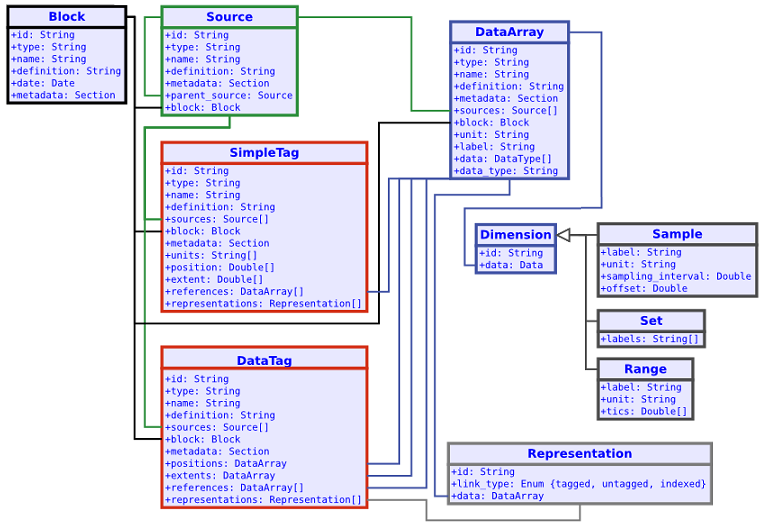
\includegraphics[scale=0.9]{obrazky/NIX_scheme.png}
	\caption{NIX data scheme. \cite{pandora}}
	\label{NIX_scheme}
\end{figure*}


This format's scheme (Figure~\ref{NIX_scheme}) served as a base format for the EEGBase file format (data in this format is finally stored in the HDF5 container) that includes the experimental data originally stored in BrainVision data format and selected metadata structures originally stored in the EEGBase Portal~\cite{eegportal}. The experimental data are stored in blocks. Each block identifies an experiment and related metadata section. Raw data (signals, stimuli) are stored in DataArrays and specified by the attributes Dimension, Sample, Set, Representation, and Range (Figure~\ref{NIX_scheme}) and could be specified by the section DataTag. The stimuli and artifacts are stored in the section SimpleTag (one stimulus) or MultiTag (more stimuli). The source for the sections DataArrays and/or Tags could be specified by the section Source. Each section could contain a~link to the metadata part that contains information about experiment.

\subsubsection{Brain Vision Format}

EEG data at University of West Bohemia is recorded by the BrainVision Recorder \cite{brainvision}. This program records raw data and saves it to three files. The BrainVision Recorder does not allow users to record data in any other format natively. The format of these files is described in the BrainVision Recorder User Manual \cite{brainUserManual}:
\begin{itemize}
	\item \textbf{data file}
	\label{eeg}
	
	This is binary file which contains recorded values from a recording device. The data are stored as double numbers.
	
	\item \textbf{vhdr file}
	\label{vhdr}
	
	This text file is Brain Vision Data Exchange Header File Version 1.0 and includes basic information about measurements. The format of the header file is based on the Windows INI format. It consists of various named sections containing key values. The file stores basic information about measuring: coding, data file name, marker file name, number of channels, sampling interval in microseconds, information about binary format (IEEE\_FLOAT\_32), and information about channels (channel number, channel name, unit, resolution of unit).
	
	\item \textbf{vmrk file}
	\label{vmrk}
	
	This is the Brain Vision Data Exchange Marker File, Version 1.0. The marker file is based upon the same principle of sections and key values as the header file is. This text file contains information about stimuli. The file stores stimuli number, type of the stimuli, stimuli description, position, size and its channel number.
	
\end{itemize}

These files are stored in the EEGBase Portal~\cite{eegportal} together with metadata describing experimental conditions.

\subsection{Hierarchical Data Format}

HDF is a data model, file format and library for storing extremely large and complex data collections. This technology is able to store any kind of data and is used all over the world in research centers and government agencies. For example, the format HDF5 is used by Cardiff University for resolving their problem with grid computing, Deutsche Bank for financial engineering, Diamond Light Source in synchrotron science, Laboratory for Neural Computation for bio-engineering and many others. A lot of formats for storing electrophysiology data use HDF5.
"The grouping structure in HDF5 enables applications to organize data objects in HDF5 to reflect complex relationships among objects. The rich collection of HDF5 datatypes, including datatypes that can point to data in other objects, and including the ability for users to define their own types, lets applications build sophisticated structures that match well with complex data. The HDF5 library has a~correspondingly rich set of operations that enables applications to access just those components that are important." \cite{hdf}


HDF is similar to XML documents, self-describing HDF files allow users to specify complex data relationships and dependencies. Several APIs for programming languages C, C++, Fortran 90, Java and others are available for this format. HDF is open-source (BSD license); stored data are human readable and the metadata model is easily customized.

\subsection{Open Metadata Markup Language}
\label{odML}

\begin{figure}[!t]
\centering
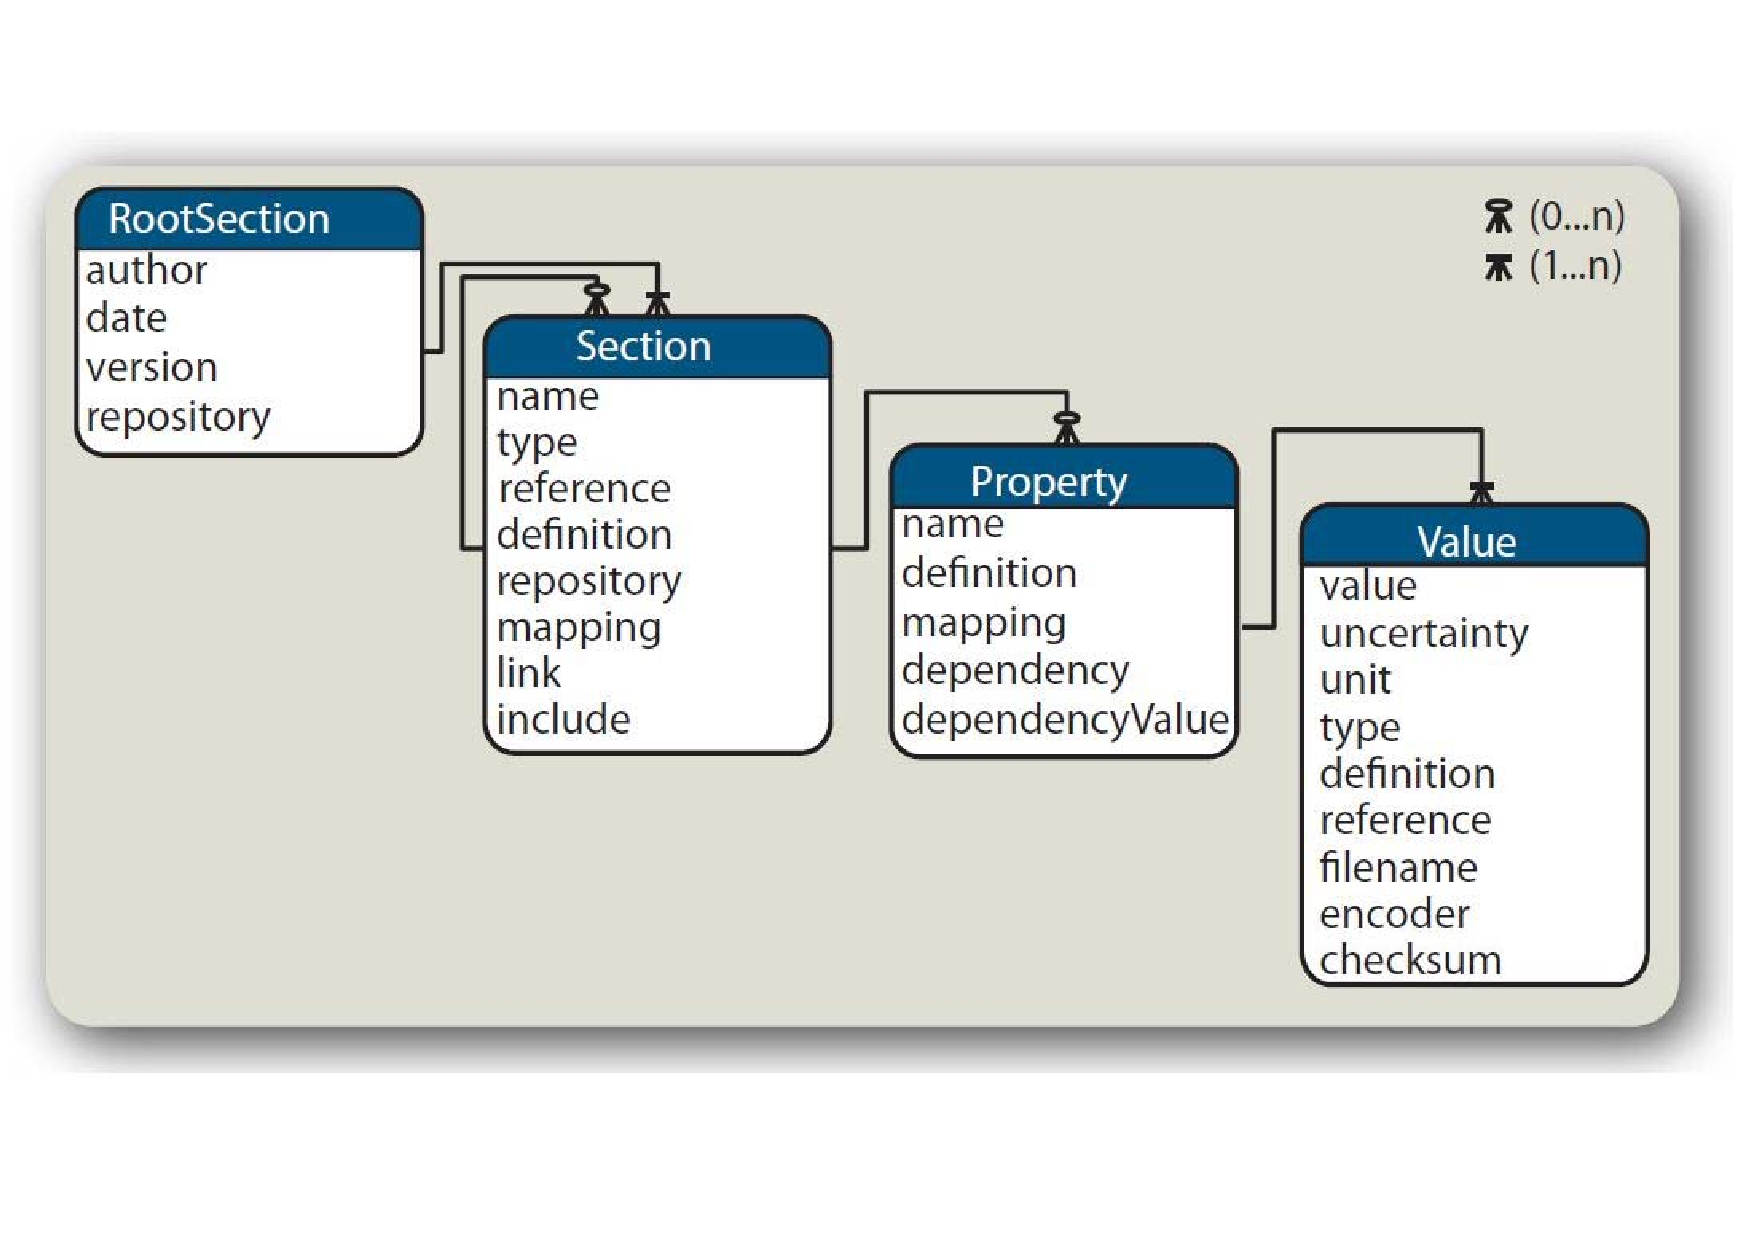
\includegraphics[scale=0.3]{obrazky/odml_tree.pdf}
\caption{Open metadata Markup Language Entity-Relation diagram. \cite{odml}}
\label{odml-tree}
\end{figure}
	
The metadata in electrophysiology domain are indispensable for the analysis and the management of experimental data within a lab. However, only rarely are metadata available in a structured, comprehensive, and machine-readable form~\cite{odml}. odML defines the format, not the content, it means that it is inherently extensible and can be adapted to the specific requirements of any laboratory. For data sharing a correct understanding of metadata and data is only possible if the same terminology is used or if mappings between terminologies are provided. For this purpose were assembled terminologies with definitions of commonly used terms.~\cite{odmlarticle}


\section{File Format Mapping and Comparison of Terminologies}

This section describes mapping of the BrainVision file format to the NIX format and comparison of odML terminology with EEGBase terminology. The EEGBase model is divided into two autonomous parts DATA and METADATA, which relate to each other, but could be read or written separately.
 
\subsubsection{Data Model}
\label{section_data}
The EEGBase data model is based on the NIX data model (Figure~\ref{NIX_scheme} and Section~\ref{nixsection}). The NIX model is able to save data from any electrophysiology experiment. However, for EEG experiments the NIX model is too general. As a result we used only the necessary parts of the model while other sections were omitted. All the omitted parts are in the NIX model optional, in this way the EEGBase data model is compatible with the NIX definition. The EEGBase data model is described in Figure~\ref{format_scheme}. It uses the NIX scheme of sections Block, DataArray, MultiTag, DataTag and SimpleTag. The section Block is used to divide measurement, the section DataArray is used for storing raw signal data and stimuli, the section MultiTag is used for storing stimuli information, and the section DataTag contains EEG channel information. DataArrays are divided into SIGNAL and MARKER parts for better transparency. The names of DataArrays also correspond to the names of channels. These adjustments allow better human readability of the file and do not influence information content at all. Metadata necessary for description of raw data form a~part of the EEGBase model (they are also included in the NIX model).   

\begin{figure}
	\begin{center}
		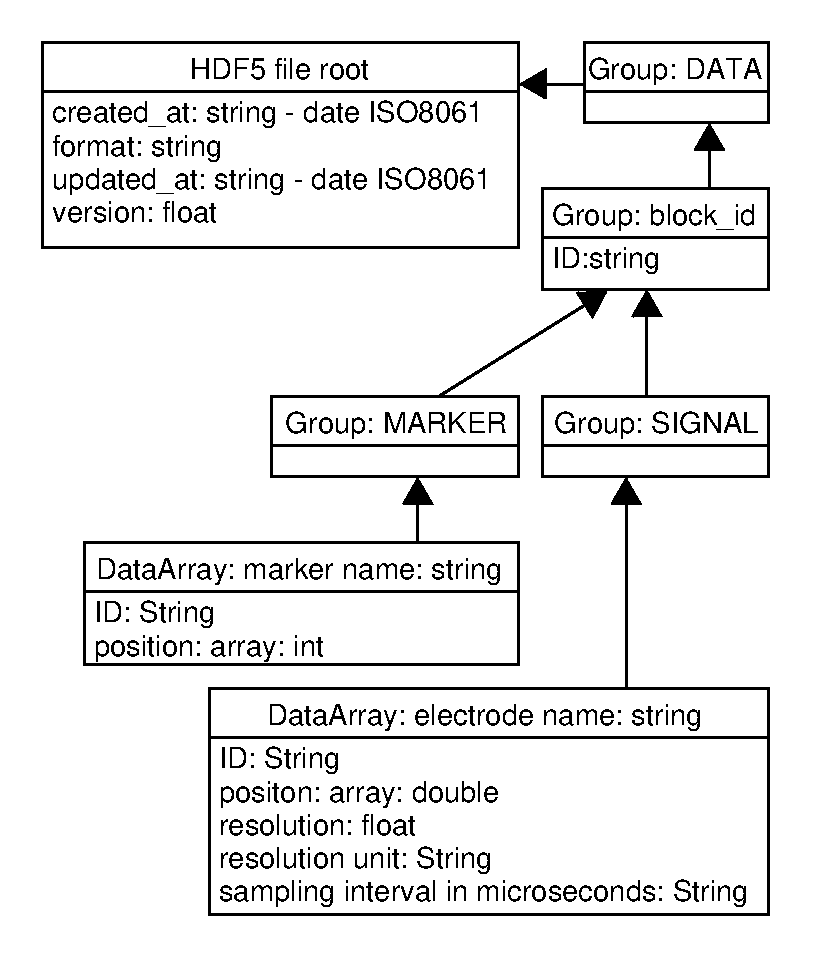
\includegraphics[scale=0.51]{obrazky/data.pdf}
		\caption{The EEGBase data model. The data are stored in a~tree structure using fixed terminology. Each Group MARKER and SIGNAL could contain zero or more DataArrays sections containing raw data.}
		\label{format_scheme}
	\end{center}
\end{figure}


\subsection{Metadata Model}
\label{odml_section}
Metadata are organized according to odML terminology. The odML scheme and terminology was used for the metadata part of file. Since the metadata scheme at UWB used terms that had not been included or not had an alternative term in the original odML terminology, this was extended with these terms. These changes and adjustments are described in Section~\ref{meta_adjustments}.

 \subsection{Metadata Terminology Extensions}
 \label{meta_adjustments}
 In order to save all our metadata into the HDF5 container we extended the odML model. These modifications were committed to G-Node INCF GitHub repository~\cite{odmlgithub}. New sections \textbf{Environment}, \textbf{Protocol} and \textbf{Software} and several attributes to the existing sections \textbf{Person} and \textbf{Electrode} were added. All suggested changes were accepted by odML developers. All modifications are listed in Table \ref{modification}.
 	\begin{savenotes}
 \begin{table}

 \caption{Modifications of the odML model.}
 	\label{modification}

 	\begin{tabular}{ | l | l | l | p{3cm} |}		
 	\hline
 \textbf{Name}& \textbf{Property} & \textbf{Value} & \textbf{Definition} \\
 	Electrode & Usage & Ground & Usage of electrode. \footnote{Added terminology that describes usage of electrode.}\\
 	\hline
 	Electrode & Usage & Reference&Usage of electrode.\footnotemark[\value{footnote}] \\
 	\hline
 	Electrode & Usage & Channel& Usage of electrode.\footnotemark[\value{footnote}]\\
 	\hline
 	Electrode & Description & String& \\
 	\hline		
 	Environment & Weather & String & \\
 	\hline	
 	Environment & RoomTemperature & String & \\
 	\hline
 	Environment & AirHumidity & float & The air humidity in \%.\\
 	\hline
 	Environment & Description & String &  \\
 	\hline
 	Protocol & Description & String & Description of the experiment\\
 	\hline
 	Protocol & Author & person & The persons who create this protocol.\\
 	\hline
 	Protocol & ProtocolFile & binary & Protocol File.\\
 	\hline
 	Protocol & ProtocolFileURL & URL & URL of protocol file.\\
 	\hline
 	Protocol & Version & String & Version of the protocol.\\
 	\hline
 	Person & Education level & String & Highest archived education level of the person.\\
 	\hline
 	Person & Role & Subject & The role of this person.\\
 	\hline
 	Person & Email & String & Person's e-mail.\\
 	\hline
 	Person & PhoneNumber & String & Person's phone number.\\
 	\hline
 	Person & Laterality & String & Handedness - The dominant hand of the subject.\\
 	\hline
 	Software & Name & String & The software name.\\
 	\hline
 	Software & Owner & String & The owner of software.\\
 	\hline
 	Software & Developer & String & Developer or developers firm of the software.\\
 	\hline
 	Software & Version & String & Version of the software.\\
 	\hline
 	Software & License & String & License type.\\
 	\hline
 	Software & LicenceStart & date & The start date of time limited license.\\ 		\hline
 	Software & LicenceExpiration & date & The end date of time limited license.\\ 		\hline
 	Software & LicenceDuration & String & Duration of the license for the software.\\ 		\hline
 	Software & LicenceCount & int & Number of the software license.\footnote{For floating licenses}\\ 		\hline
 	Software & Distribution & String & Distribution type.\\ 		\hline
 	Software & Description & String & \\ 		\hline
 	Software & LicenceDuration & String & Duration of the license for the software.\\ 		\hline
 \end{tabular}

 \end{table}
 \end{savenotes}
 
\section{HDFExport Program}

This section deals with design and implementation of HDFExport program that converts the BrainVision file format data and EEGBase portal metadata into the HDF5 container.

\subsubsection {Use Cases}
The HDFExport program is designed for several use cases that could be divided by data and metadata location (Figure~\ref{use_case1}):
\begin{itemize}
	\item data and metadata export from locally stored Brain Vision files only,
	\item data and metadata export from locally stored Brain Vision files and metadata from EEGBase portal,
	\item data and basic metadata export from in EEGBase postal stored Brain Vision files without experiments metadata,
	\item data and metadata export from EEGBase portal and Brain Vision files stored in EEGBase portal
\end{itemize}

\begin{figure}
	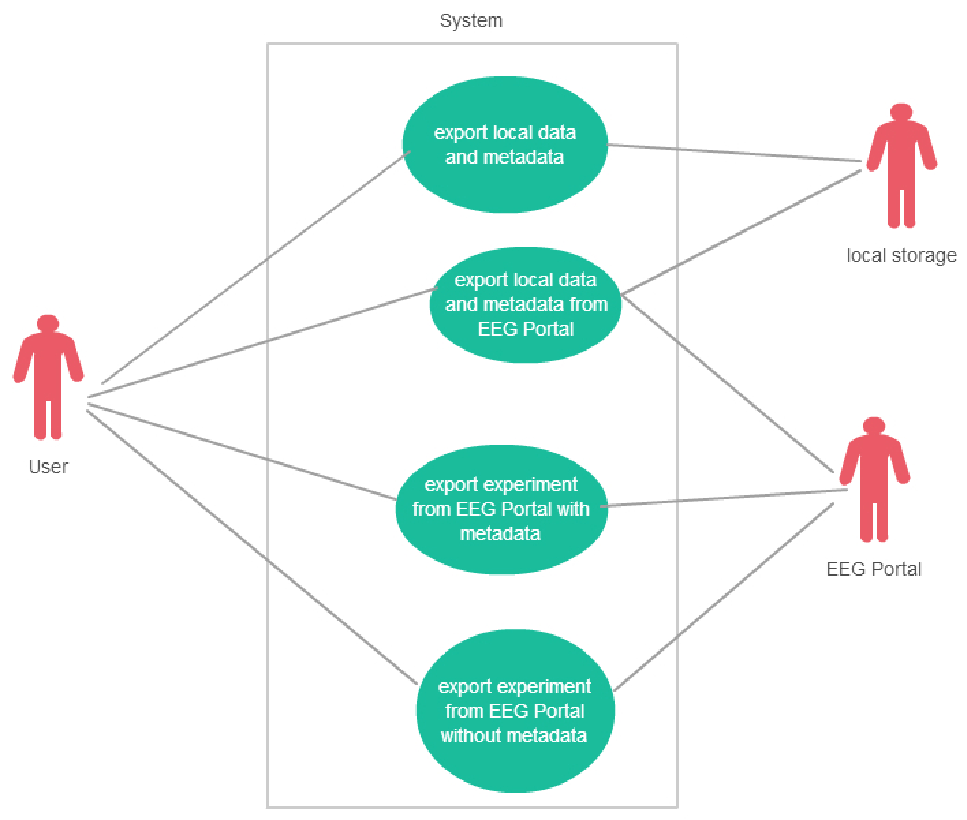
\includegraphics[scale=0.5]{obrazky/use_case_location.pdf}	
	\caption{Use cases of HDFExport Program.}
	\label{use_case1}
\end{figure}
We can also divide use cases according to the type of exported data (Figure~\ref{use_case2}):
\begin{itemize}
	\item Only raw EEG data and basic metadata are exported.
	
	Only data and metadata from the Brain Vision files are exported. Stimuli are not exported (not all measurements uses stimuli).
	\item Raw EEG data, basic metadata and stimuli are exported.
	
	All data, metadata and stimuli from Brain Vision files are exported.
	\item Raw EEG data, basic metadata, stimuli and experiments metadata are exported.
	
	All data, metadata and stimuli from the Brain Vision files and experiments metadata from EEGBase portal are exported.
	\item Raw EEG data, basic metadata and experiments information are exported.
	
	All data, metadata and experiments information are exported.
\end{itemize}
\begin{figure}
	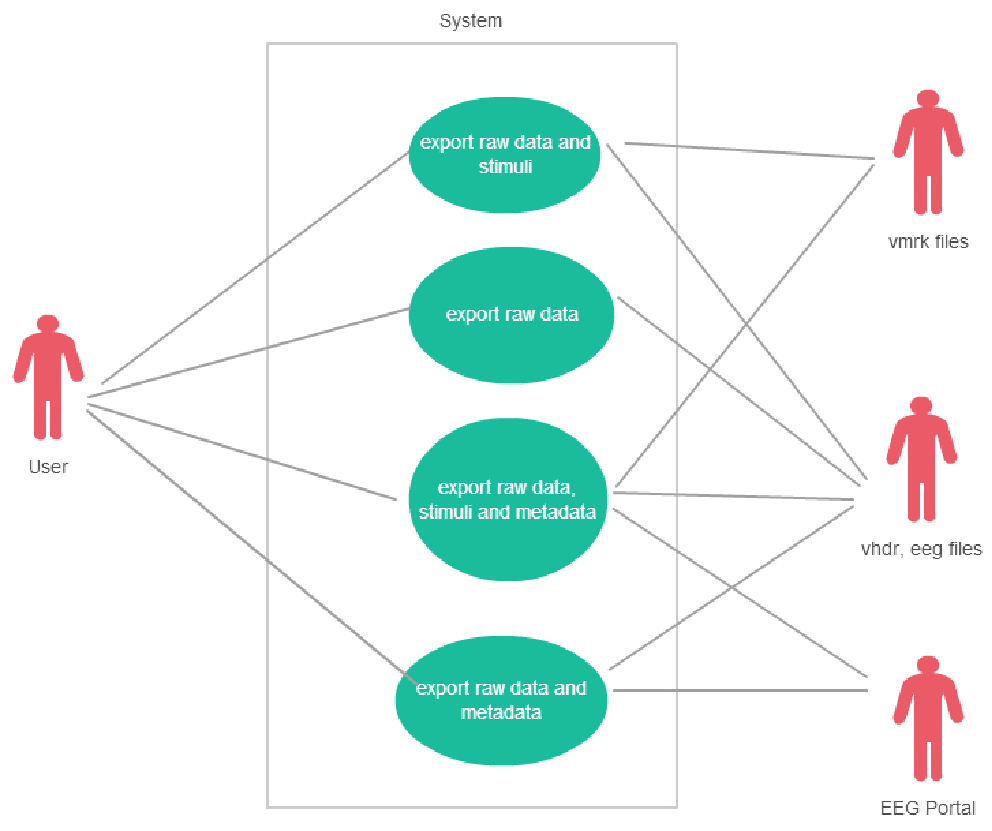
\includegraphics[scale=0.5]{obrazky/use_case_data.pdf}	
	\caption{Use cases of HDFExport Program.}
	\label{use_case2}
\end{figure}


\subsubsection {Implementation}

Java was selected as a programming language for program developing, since there already exists a~parser of Brain Vision formats developed. Moreover, the EEGBase portal is written in Java. There is an effort to include the export program into the EEGBase portal for easy export.

%\begin{figure*}
%	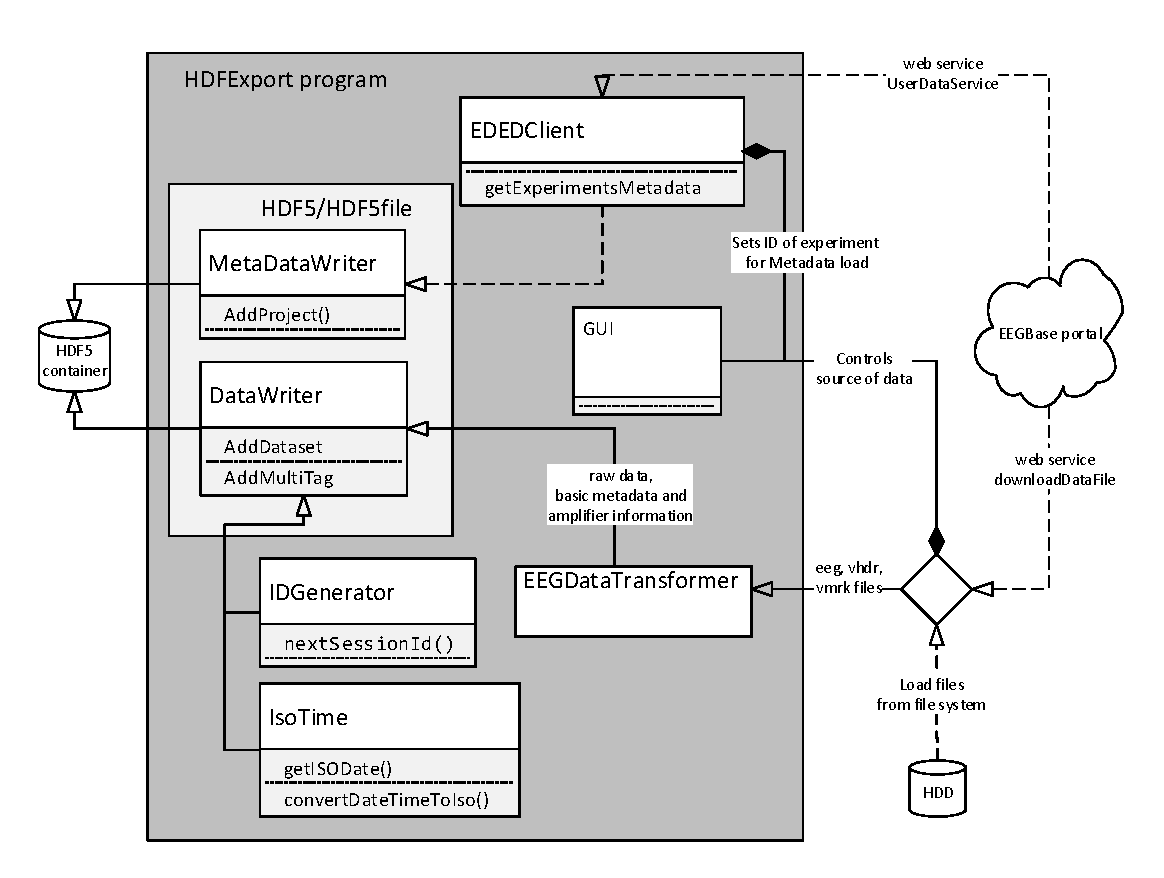
\includegraphics[scale=0.73]{obrazky/ExportProgramDiagram.pdf}	
%	\caption{The diagram of EEGBase HDF5 export program}
%	\label{export-diagram}
%\end{figure*}
\section{Tests}

The program was manually tested for several use cases and all created HDF5 files were verified manually (they were opened and the contents was checked) by the program provided by the HDF Group, HDFView \cite{hdfjava} in version 2.11. 

\subsection{Performance Tests}

The write performance tests were conducted to determine time consumption of export. The tests were run on a~standard desktop computer (Intel Core i7 at 3,4 GHz, 8 GB of DDR3 RAM, standard HDD with 7200 rpm). An unusually high memory consumption was detected during the test. The amount of occupied memory by the EEGExport program for big (220 MB) experimental data reached up to 4 GB of memory. Further testing showed that Java Virtual Machine, in attempt to speed up export, did not free allocated memory. However, when the program was paused, the size of allocated memory became lower. Finally, the disk writing speed was a limited factor. The conversion times with GZip compression are shown in Table~\ref{speed_test}. The GZip compression was used to reduce file size. The GZip compression is integrated in HDF libraries and it is supported natively (reading of the data does not require any special actions).

\begin{table}
	\catcode`\-=12
	\centering
	\caption{Performance tests with GZip compression. Each file was saved seven times.}
	\label{speed_test}
	\begin{tabular}{|c|c|c|c|c|}
		\hline
		\textbf{File size} & \multicolumn{4}{c|}{\textbf{Time needed for conversion in ms}}\\
		\cline{2-5}		
		\textbf{ of Brain Vision files}	&\textbf{Best} & \textbf{Worst} & \textbf{Average} & \textbf{With compression}\\
		\hline
		\hline 21,3 MB & 3010 & 3501  & 3132& 7529 \\ 	
		\hline 51,2 MB & 6160  & 7906 & 6700 & 26051\\
		\hline 58 MB & 7668 &  8262 &  7947& 29032\\
		\hline 87,2 MB & 31364 & 35957 & 32820& 44877\\
		\hline 197,8 MB & 13060  & 14625 &  13502& 40168\\ 		
		\hline 221,3 MB & 14589 & 16321 & 15197& 42679 \\
		\hline 221,6 MB & 14347  & 16108 & 14871& 43586\\
		\hline
	\end{tabular}
\end{table}


\subsection{File Size Tests}
Several file size tests were conducted to determine the resulting file size of the HDF5 container storing all data. Data from real experiments were used for the tests. The test showed that the size of the HDF5 container was influenced by exported data and the original file size was not the only decisive factor. The size of the HDF5 container was always bigger than Brain Vision files, four times bigger at the worst case, two times at the best case. The results are shown in Table~\ref{file_size}. 

\begin{table}[h]
	\caption{File size tests.}
	\label{file_size}
	\centering
	\begin{tabular}{|c|c|c|c|}
		\hline \textbf{File size}  & {\textbf{HDF5 file size}}& {\textbf{HDF5 file size}}  & \textbf{Ratio}	\\
		\textbf{of Brain Vision files} & &  with compression &	\\
		\hline 21,3 MB & 80,9 MB & 26,92 MB& 1,26x\\
		\hline 51,2 MB & 194,2 MB & 112,98 MB & 2,21x\\
		\hline 58 MB & 221,1 MB & 102,79 MB & 1,77x\\
		\hline 87,2 MB & 329,7 MB & 124,51 MB & 1,43x\\
		\hline 197,8 MB & 370,9 MB & 305,19 MB& 1,54x\\ 		
		\hline 221,3 MB & 414,9 MB & 355,58 MB & 1,61x\\
		\hline 221,6 MB & 415,5 MB & 334,46 MB & 1,51x\\ 		
		\hline
	\end{tabular}
\end{table}

\begin{table}
	\caption{File size dependency on compression chunk size.}
	\label{chunk_size}
	\centering
	\begin{tabular}{|c|c|c|c|c|}
		\hline {\textbf{Original file size}}  & \multicolumn{4}{ c| }{\textbf{HDF5 file size in MB}}\\
		& chunk 64 & chunk 256 & chunk 512 &  chunk 1024	\\
		\hline 21,3 MB &  39,76  & 26,92 & 23,30 & 20,46\\ 	
		\hline 51,2 MB & 155,47 & 112,98  & 99,31 & 87,85 \\
		\hline 58 MB    & 151,31 & 102,79 & 88,60 & 77,96 \\
		\hline 87,2 MB & 176,53  & 124,51 &  112,43& 104,15\\
		\hline 197,8 MB & 365,63 & 305,19 & 292,59 & 285,48\\ 		
		\hline 221,3 MB & 422,83  & 355,58& 341,72 & 333,83\\
		\hline 221,6 MB & 402,81 & 334,46 & 320,22 & 312,10 \\
		\hline
	\end{tabular}
\end{table}



\section{Conclusion}
We examined current file formats for storing electrophysiology data and data from experiments and measurements conducted at the University of West Bohemia. We became familiar with the data and metadata model of EEG measurements and its terminology. We examined the data and metadata model of EEGBase portal.

We analyzed two early file standard proposals from INCF and I tracked progress in both. We found several currently used formats, which are using HDF as a container in neuroinformatics. We chose the most suitable format for our data and usage considering INCF recommendations.

We created implementation of the chosen format. We chose HDF5 container for the EEGBase format. We joined the INCF Electrophysiology Data Sharing Task Force and contributed to the odML terminology. We developed a program that transforms raw data and metadata from Brain Vision files to the EEGBase format, and We also included metadata which are stored in the EEGBase portal. We tested my format and program for several use cases and its performance.

The proposed EEGBase format is capable of storing all currently saved data and metadata and is able to store the future changes and modifications of metadata model. The developed program stores measured data into the EEGBase format. I also made a few suggestions for the UWB model. The program is currently using web services of the EEGBase portal for metadata loading. The developed libraries allow export of raw data or data with metadata. Exporting experimental data and metadata in the EEGBase format to the HDF5 container improves sharing capabilities of the EEGBase portal and overall attractiveness of stored experiments.





% conference papers do not normally have an appendix







% trigger a \newpage just before the given reference
% number - used to balance the columns on the last page
% adjust value as needed - may need to be readjusted if
% the document is modified later
%\IEEEtriggeratref{8}
% The "triggered" command can be changed if desired:
%\IEEEtriggercmd{\enlargethispage{-5in}}

% references section

% can use a bibliography generated by BibTeX as a .bbl file
% BibTeX documentation can be easily obtained at:
% http://www.ctan.org/tex-archive/biblio/bibtex/contrib/doc/
% The IEEEtran BibTeX style support page is at:
% http://www.michaelshell.org/tex/ieeetran/bibtex/
%\bibliographystyle{IEEEtran}
% argument is your BibTeX string definitions and bibliography database(s)
%\bibliography{IEEEabrv,../bib/paper}
%
% <OR> manually copy in the resultant .bbl file
% set second argument of \begin to the number of references
% (used to reserve space for the reference number labels box)

\begin{thebibliography}{1}


\bibitem{Poldrack2012}
{\sc Poldrack}, R.~A.
\newblock The future of {fMRI} in cognitive neuroscience.
\newblock \emph{{NeuroImage}}. aug 2012, 62, 2, s.~1216--1220.
\newblock \texttt{10.1016/j.neuroimage.2011.08.007}.
\newblock Available from:
$\texttt{{http://dx.doi.org/10.1016/j.neuroimage.2011.08.007}}$.

\bibitem{Milham2012}
{\sc Milham}, M.~P.
\newblock Open Neuroscience Solutions for the Connectome-wide Association Era.
\newblock \emph{Neuron}. jan 2012, 73, 2, s.~214--218.
\newblock \texttt{10.1016/j.neuron.2011.11.004}.
\newblock Available from:
$\texttt{{http://dx.doi.org/10.1016/j.neuron.2011.11.004}}$.

\bibitem{Poline2012}
{\sc Poline}, J.-B. et~al.
\newblock Data sharing in neuroimaging research.
\newblock \emph{Frontiers in Neuroinformatics}. 2012, 6.
\newblock \texttt{10.3389/fninf.2012.00009}.
\newblock Available from:
$\texttt{{http://dx.doi.org/10.3389/fninf.2012.00009}}$.

\bibitem{incf_mission}
{\sc Friedrich}, S. et~al.
\newblock Mission and activities of the {INCF} Electrophysiology Data Sharing
Task Force.
\newblock \emph{Frontiers in Neuroinformatics}. 2014, 8.
\newblock \texttt{10.3389/conf.fninf.2014.08.00088}.
\newblock Available from:
$\texttt{{http://dx.doi.org/10.3389/conf.fninf.2014.08.00088}}$.


\bibitem{eegportal}
\emph{EEGbase} [online]. 2015. [cit.~10.5.2015]. RRID:nif-0000-08190.
\newblock Available from: $\texttt{{https://eegdatabase.kiv.zcu.cz/}}$.


\bibitem{hdfjava}
\emph{HDF Java Products} [online]. 2014. [cit.~1.5.2015]. HDF Group.
\newblock Available from: $\texttt{{https://www.hdfgroup.org/products/java/}}$.



\bibitem{odmlgithub}
\emph{INCF GitHub odML repository} [online]. [cit.~12.5.2015].
\newblock Available from:
$\texttt{{https://github.com/INCF/odml-terminologies}}$.


\bibitem{requirements}
Requirements for storing electrophysiology data, Version 0.72.
\newblock Available from: $\texttt{{https://goo.gl/QbClkE}}$.
\newblock Electrophysiology Task Force of the INCF Program on Standards for
Data Sharing, 2014.

\bibitem{odmlarticle}
{\sc Benda}, J.
\newblock From recording to sharing of data - embedding metadata handling into
the laboratory workflow using {odML}.
\newblock \emph{Frontiers in Neuroinformatics}. 2011, 5.
\newblock \texttt{10.3389/conf.fninf.2011.08.00100}.
\newblock Available from:
$\texttt{{http://dx.doi.org/10.3389/conf.fninf.2011.08.00100}}$.

\bibitem{brainUserManual}
Brain Products GmbH.
\newblock \emph{BrainVision Recorder User Manual}.
\newblock Brain Products GmbH, 011 edition, December 2014.

\bibitem{brainvision}
\emph{Brain Products GmbH} [online]. 2014. [cit.~03.07.2014].
Brain Products GmbH.
\newblock Available from: $\texttt{{http://www.brainproducts.com/index.php}}$.



\bibitem{Brinkman2010}
{\sc Brinkman}, R.~R. et~al.
\newblock Modeling biomedical experimental processes with {OBI}.
\newblock \emph{Journal of Biomedical Semantics}. 2010, 1, Suppl 1, s.~S7.
\newblock \texttt{10.1186/2041-1480-1-s1-s7}.
\newblock Available from:
$\texttt{{http://dx.doi.org/10.1186/2041-1480-1-S1-S7}}$.



\bibitem{incf_mission}
{\sc Friedrich}, S. et~al.
\newblock Mission and activities of the {INCF} Electrophysiology Data Sharing
Task Force.
\newblock \emph{Frontiers in Neuroinformatics}. 2014, 8.
\newblock \texttt{10.3389/conf.fninf.2014.08.00088}.
\newblock Available from:
$\texttt{{http://dx.doi.org/10.3389/conf.fninf.2014.08.00088}}$.



\bibitem{odml}
{\sc Grewe}, J. -- {\sc Wachtler}, T. -- {\sc Benda}, J.
\newblock A Bottom-up Approach to Data Annotation in Neurophysiology.
\newblock \emph{Frontiers in Neuroinformatics}. 2011, 5.
\newblock \texttt{10.3389/fninf.2011.00016}.
\newblock Available from:
$\texttt{{http://dx.doi.org/10.3389/fninf.2011.00016}}$.

\bibitem{hdf}
\emph{HDF Technologies} [online]. 2013. [cit.~03.07.2014]. The HDF Group.
\newblock Available from: $\texttt{{http://www.hdfgroup.org/}}$.

\bibitem{incfweb}
\emph{INCF} [online]. 2015. [cit.~4.3.2015].
\newblock Available from: $\texttt{{http://www.incf.org/}}$.

\bibitem{incfwebtaskforce}
\emph{INCF} [online]. 2015. [cit.~4.3.2015].
\newblock Available from: $\texttt{{http://www.incf.org/activities/our-programs/datasharing/electrophysiology-task-force/}}$.

%\bibitem{ephdf}
%{\sc Jeffrey}, T. -- {\sc Friedrich}, S.
%\newblock {epHDF} {\textendash} a proposed standard for storing
%electrophysiology data in {HDF}5.
%\newblock \emph{Frontiers in Neuroinformatics}. 2013, 7.
%\newblock \texttt{10.3389/conf.fninf.2013.09.00068}.
%\newblock Available from:
%$\texttt{{http://dx.doi.org/10.3389/conf.fninf.2013.09.00068}}$.



\bibitem{kemp2003}
{\sc Kemp}, B. -- {\sc Olivan}, J.
\newblock European data format `plus' (EDF+), an {EDF} alike standard format
for the exchange of physiological data.
\newblock \emph{Clinical Neurophysiology}. sep 2003, 114, 9, s.~1755--1761.
\newblock \texttt{10.1016/s1388-2457(03)00123-8}.
\newblock Available from:
$\texttt{{http://dx.doi.org/10.1016/S1388-2457(03)00123-8}}$.




\bibitem{Milham2012}
{\sc Milham}, M.~P.
\newblock Open Neuroscience Solutions for the Connectome-wide Association Era.
\newblock \emph{Neuron}. jan 2012, 73, 2, s.~214--218.
\newblock \texttt{10.1016/j.neuron.2011.11.004}.
\newblock Available from:
$\texttt{{http://dx.doi.org/10.1016/j.neuron.2011.11.004}}$.

\bibitem{neo}
\emph{Neo} [online]. 2014. [cit.~03.07.2014].
\newblock Available from: $\texttt{{http://pythonhosted.org/neo/}}$.

\bibitem{neurohdf}
\emph{NeuroHDF} [online]. 2014. [cit.~03.07.2014]. NeuroHDF Interest Group.
\newblock Available from: $\texttt{{https://neurohdf.readthedocs.org/}}$.

\bibitem{nexus}
\emph{NeXus Format} [online]. 2014. [cit.~03.07.2014]. NeXus International
Advisory Committee.
\newblock Available from: $\texttt{{http://www.nexusformat.org/}}$.




\bibitem{Poldrack2012}
{\sc Poldrack}, R.~A.
\newblock The future of {fMRI} in cognitive neuroscience.
\newblock \emph{{NeuroImage}}. aug 2012, 62, 2, s.~1216--1220.
\newblock \texttt{10.1016/j.neuroimage.2011.08.007}.
\newblock Available from:
$\texttt{{http://dx.doi.org/10.1016/j.neuroimage.2011.08.007}}$.



\bibitem{pandora}
\emph{NIX} [online]. 2014. [cit.~03.02.2015]. G-Node.
\newblock Available from: $\texttt{{https://github.com/G-Node/nix/wiki}}$.

\bibitem{ovation}
\emph{Ovation} [online]. 2014. [cit.~3.7.2014]. Physion LLC.
\newblock Available from: $\texttt{{http://physion.us/}}$.


\bibitem{oen}
\emph{The Open Biological and Biomedical Ontologies} [online]. 2015.
[cit.~10.5.2015].
\newblock Available from: $\texttt{{http://www.obofoundry.org/}}$.
\end{thebibliography}




% that's all folks
\end{document}


